\documentclass{standalone}
\usepackage{tikz}
\usetikzlibrary{patterns, positioning}

\begin{document}
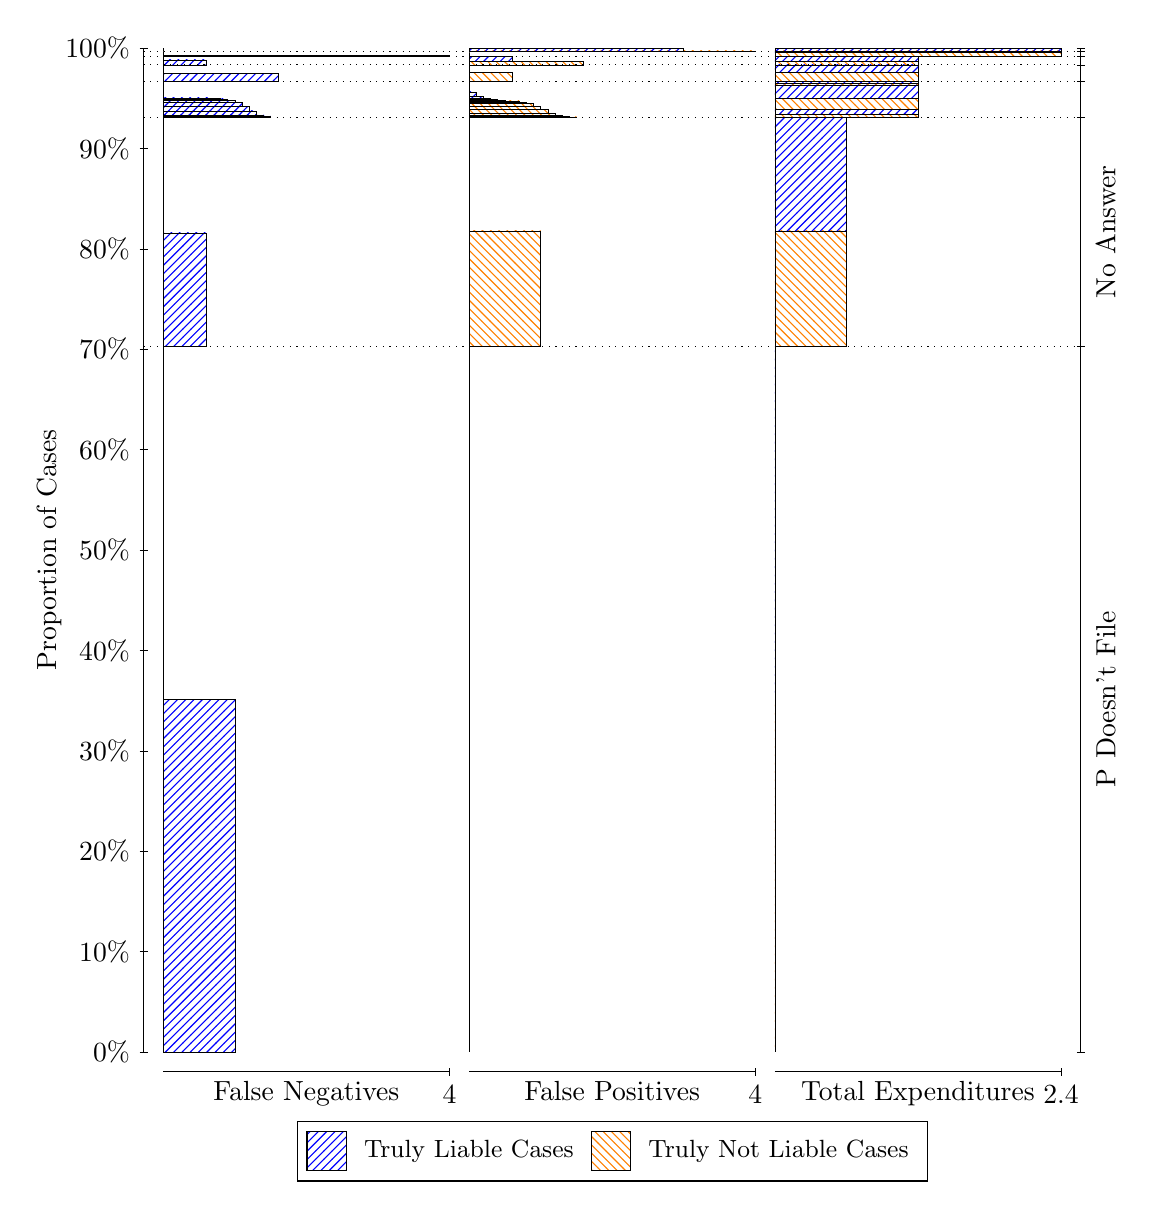
\begin{tikzpicture}
\draw[black, very thin] (1.5,1.75) -- (1.5,14.5);
\node[rotate=90, anchor=center] at (0.3, 8.125) {Proportion of Cases};
\draw[black, very thin] (1.45,1.75) -- (1.55,1.75);
\node[anchor=east] at (1.45, 1.75) {0\%};
\draw[black, very thin] (1.45,3.025) -- (1.55,3.025);
\node[anchor=east] at (1.45, 3.025) {10\%};
\draw[black, very thin] (1.45,4.3) -- (1.55,4.3);
\node[anchor=east] at (1.45, 4.3) {20\%};
\draw[black, very thin] (1.45,5.575) -- (1.55,5.575);
\node[anchor=east] at (1.45, 5.575) {30\%};
\draw[black, very thin] (1.45,6.85) -- (1.55,6.85);
\node[anchor=east] at (1.45, 6.85) {40\%};
\draw[black, very thin] (1.45,8.125) -- (1.55,8.125);
\node[anchor=east] at (1.45, 8.125) {50\%};
\draw[black, very thin] (1.45,9.4) -- (1.55,9.4);
\node[anchor=east] at (1.45, 9.4) {60\%};
\draw[black, very thin] (1.45,10.675) -- (1.55,10.675);
\node[anchor=east] at (1.45, 10.675) {70\%};
\draw[black, very thin] (1.45,11.95) -- (1.55,11.95);
\node[anchor=east] at (1.45, 11.95) {80\%};
\draw[black, very thin] (1.45,13.225) -- (1.55,13.225);
\node[anchor=east] at (1.45, 13.225) {90\%};
\draw[black, very thin] (1.45,14.5) -- (1.55,14.5);
\node[anchor=east] at (1.45, 14.5) {100\%};

\draw[black, very thin] (13.4,1.75) -- (13.4,14.5);
\draw[black, very thin] (13.35,1.75) -- (13.45,1.75);
\node[anchor=west] at (13.35, 1.75) {};
\draw[black, very thin] (13.35,10.713) -- (13.45,10.713);
\node[anchor=west] at (13.35, 10.713) {};
\draw[black, very thin] (13.35,13.619) -- (13.45,13.619);
\node[anchor=west] at (13.35, 13.619) {};
\draw[black, very thin] (13.35,14.08) -- (13.45,14.08);
\node[anchor=west] at (13.35, 14.08) {};
\draw[black, very thin] (13.35,14.287) -- (13.45,14.287);
\node[anchor=west] at (13.35, 14.287) {};
\draw[black, very thin] (13.35,14.394) -- (13.45,14.394);
\node[anchor=west] at (13.35, 14.394) {};
\draw[black, very thin] (13.35,14.453) -- (13.45,14.453);
\node[anchor=west] at (13.35, 14.453) {};
\draw[black, very thin] (13.35,14.5) -- (13.45,14.5);
\node[anchor=west] at (13.35, 14.5) {};

\draw[black, very thin, pattern color=blue, pattern=north east lines] (1.75,1.75) rectangle (2.6583,6.2313);
\draw[black, very thin, pattern color=orange, pattern=north west lines] (1.75,6.2313) rectangle (1.75,10.713);
\draw[black, very thin, pattern color=blue, pattern=north east lines] (1.75,10.713) rectangle (2.295,12.152);
\draw[black, very thin, pattern color=orange, pattern=north west lines] (1.75,12.152) rectangle (1.75,13.619);
\draw[black, very thin, pattern color=blue, pattern=north east lines] (1.75,13.619) rectangle (3.1125,13.637);
\draw[black, very thin, pattern color=blue, pattern=north east lines] (1.75,13.637) rectangle (3.0217,13.651);
\draw[black, very thin, pattern color=blue, pattern=north east lines] (1.75,13.651) rectangle (2.9308,13.703);
\draw[black, very thin, pattern color=blue, pattern=north east lines] (1.75,13.703) rectangle (2.84,13.757);
\draw[black, very thin, pattern color=blue, pattern=north east lines] (1.75,13.757) rectangle (2.7492,13.809);
\draw[black, very thin, pattern color=blue, pattern=north east lines] (1.75,13.809) rectangle (2.6583,13.836);
\draw[black, very thin, pattern color=blue, pattern=north east lines] (1.75,13.836) rectangle (2.5675,13.854);
\draw[black, very thin, pattern color=blue, pattern=north east lines] (1.75,13.854) rectangle (2.4767,13.861);
\draw[black, very thin, pattern color=blue, pattern=north east lines] (1.75,13.861) rectangle (2.3858,13.868);
\draw[black, very thin, pattern color=orange, pattern=north west lines] (1.75,13.868) rectangle (1.75,14.08);
\draw[black, very thin, pattern color=blue, pattern=north east lines] (1.75,14.08) rectangle (3.2033,14.174);
\draw[black, very thin, pattern color=orange, pattern=north west lines] (1.75,14.174) rectangle (1.75,14.287);
\draw[black, very thin, pattern color=blue, pattern=north east lines] (1.75,14.287) rectangle (2.295,14.35);
\draw[black, very thin, pattern color=orange, pattern=north west lines] (1.75,14.35) rectangle (1.75,14.394);
\draw[black, very thin, pattern color=blue, pattern=north east lines] (1.75,14.394) rectangle (5.3833,14.404);
\draw[black, very thin, pattern color=orange, pattern=north west lines] (1.75,14.404) rectangle (1.75,14.453);
\draw[black, very thin, pattern color=orange, pattern=north west lines] (1.75,14.453) rectangle (1.75,14.463);
\draw[black, very thin, pattern color=blue, pattern=north east lines] (1.75,14.463) rectangle (1.75,14.5);
\draw[black, very thin, pattern color=orange, pattern=north west lines] (5.6333,1.75) rectangle (5.6333,6.2314);
\draw[black, very thin, pattern color=blue, pattern=north east lines] (5.6333,6.2314) rectangle (5.6333,10.713);
\draw[black, very thin, pattern color=orange, pattern=north west lines] (5.6333,10.713) rectangle (6.5417,12.179);
\draw[black, very thin, pattern color=blue, pattern=north east lines] (5.6333,12.179) rectangle (5.6333,13.619);
\draw[black, very thin, pattern color=orange, pattern=north west lines] (5.6333,13.619) rectangle (6.9958,13.625);
\draw[black, very thin, pattern color=orange, pattern=north west lines] (5.6333,13.625) rectangle (6.905,13.632);
\draw[black, very thin, pattern color=orange, pattern=north west lines] (5.6333,13.632) rectangle (6.8142,13.649);
\draw[black, very thin, pattern color=orange, pattern=north west lines] (5.6333,13.649) rectangle (6.7233,13.674);
\draw[black, very thin, pattern color=orange, pattern=north west lines] (5.6333,13.674) rectangle (6.6325,13.719);
\draw[black, very thin, pattern color=orange, pattern=north west lines] (5.6333,13.719) rectangle (6.5417,13.761);
\draw[black, very thin, pattern color=orange, pattern=north west lines] (5.6333,13.761) rectangle (6.4508,13.797);
\draw[black, very thin, pattern color=orange, pattern=north west lines] (5.6333,13.797) rectangle (6.36,13.806);
\draw[black, very thin, pattern color=orange, pattern=north west lines] (5.6333,13.806) rectangle (6.2692,13.83);
\draw[black, very thin, pattern color=blue, pattern=north east lines] (5.6333,13.83) rectangle (6.0875,13.837);
\draw[black, very thin, pattern color=blue, pattern=north east lines] (5.6333,13.837) rectangle (5.9967,13.845);
\draw[black, very thin, pattern color=blue, pattern=north east lines] (5.6333,13.845) rectangle (5.9058,13.862);
\draw[black, very thin, pattern color=blue, pattern=north east lines] (5.6333,13.862) rectangle (5.815,13.889);
\draw[black, very thin, pattern color=blue, pattern=north east lines] (5.6333,13.889) rectangle (5.7242,13.942);
\draw[black, very thin, pattern color=blue, pattern=north east lines] (5.6333,13.942) rectangle (5.6333,14.08);
\draw[black, very thin, pattern color=orange, pattern=north west lines] (5.6333,14.08) rectangle (6.1783,14.193);
\draw[black, very thin, pattern color=blue, pattern=north east lines] (5.6333,14.193) rectangle (5.6333,14.287);
\draw[black, very thin, pattern color=orange, pattern=north west lines] (5.6333,14.287) rectangle (7.0867,14.331);
\draw[black, very thin, pattern color=blue, pattern=north east lines] (5.6333,14.331) rectangle (6.1783,14.394);
\draw[black, very thin, pattern color=orange, pattern=north west lines] (5.6333,14.394) rectangle (5.6333,14.443);
\draw[black, very thin, pattern color=blue, pattern=north east lines] (5.6333,14.443) rectangle (5.6333,14.453);
\draw[black, very thin, pattern color=orange, pattern=north west lines] (5.6333,14.453) rectangle (9.2667,14.463);
\draw[black, very thin, pattern color=blue, pattern=north east lines] (5.6333,14.463) rectangle (8.3583,14.5);
\draw[black, very thin, pattern color=orange, pattern=north west lines] (9.5167,1.75) rectangle (9.5167,6.2314);
\draw[black, very thin, pattern color=blue, pattern=north east lines] (9.5167,6.2314) rectangle (9.5167,10.713);
\draw[black, very thin, pattern color=orange, pattern=north west lines] (9.5167,10.713) rectangle (10.425,12.179);
\draw[black, very thin, pattern color=blue, pattern=north east lines] (9.5167,12.179) rectangle (10.425,13.619);
\draw[black, very thin, pattern color=orange, pattern=north west lines] (9.5167,13.619) rectangle (11.333,13.664);
\draw[black, very thin, pattern color=blue, pattern=north east lines] (9.5167,13.664) rectangle (11.333,13.716);
\draw[black, very thin, pattern color=orange, pattern=north west lines] (9.5167,13.716) rectangle (11.333,13.859);
\draw[black, very thin, pattern color=blue, pattern=north east lines] (9.5167,13.859) rectangle (11.333,14.031);
\draw[black, very thin, pattern color=orange, pattern=north west lines] (9.5167,14.031) rectangle (11.333,14.054);
\draw[black, very thin, pattern color=blue, pattern=north east lines] (9.5167,14.054) rectangle (11.333,14.08);
\draw[black, very thin, pattern color=orange, pattern=north west lines] (9.5167,14.08) rectangle (11.333,14.193);
\draw[black, very thin, pattern color=blue, pattern=north east lines] (9.5167,14.193) rectangle (11.333,14.287);
\draw[black, very thin, pattern color=orange, pattern=north west lines] (9.5167,14.287) rectangle (11.333,14.331);
\draw[black, very thin, pattern color=blue, pattern=north east lines] (9.5167,14.331) rectangle (11.333,14.394);
\draw[black, very thin, pattern color=orange, pattern=north west lines] (9.5167,14.394) rectangle (13.15,14.443);
\draw[black, very thin, pattern color=blue, pattern=north east lines] (9.5167,14.443) rectangle (13.15,14.453);
\draw[black, very thin, pattern color=orange, pattern=north west lines] (9.5167,14.453) rectangle (13.15,14.463);
\draw[black, very thin, pattern color=blue, pattern=north east lines] (9.5167,14.463) rectangle (13.15,14.5);
\draw[black, dotted] (1.5,10.713) -- (13.4,10.713);
\draw[black, dotted] (1.5,13.619) -- (13.4,13.619);
\draw[black, dotted] (1.5,14.08) -- (13.4,14.08);
\draw[black, dotted] (1.5,14.287) -- (13.4,14.287);
\draw[black, dotted] (1.5,14.394) -- (13.4,14.394);
\draw[black, dotted] (1.5,14.453) -- (13.4,14.453);
\draw[black, very thin] (1.75,1.5) -- (5.3833,1.5);
\node[anchor=north] at (3.5667, 1.5) {False Negatives};
\draw[black, very thin] (5.3833,1.45) -- (5.3833,1.55);
\node[anchor=north] at (5.3833, 1.45) {4};

\draw[black, very thin] (5.6333,1.5) -- (9.2667,1.5);
\node[anchor=north] at (7.45, 1.5) {False Positives};
\draw[black, very thin] (9.2667,1.45) -- (9.2667,1.55);
\node[anchor=north] at (9.2667, 1.45) {4};

\draw[black, very thin] (9.5167,1.5) -- (13.15,1.5);
\node[anchor=north] at (11.333, 1.5) {Total Expenditures};
\draw[black, very thin] (13.15,1.45) -- (13.15,1.55);
\node[anchor=north] at (13.15, 1.45) {2.4};

\node[black, centered, rotate=90] at (13.72, 6.2313) {P Doesn't File};
\node[black, centered, rotate=90] at (13.72, 12.166) {No Answer};






\draw (7.449999999999999,1.5) node[draw=none] (baseCoordinate) {};
\begin{scope}[align=center]
        \matrix[scale=0.5, draw=black, below=0.5cm of baseCoordinate, nodes={draw}, column sep=0.1cm]{
            \node[rectangle, draw, minimum width=0.5cm, minimum height=0.5cm, pattern=north east lines, pattern color=blue] {}; &
            \node[draw=none, font=\small] (B) {Truly Liable Cases}; &
            \node[rectangle, draw, minimum width=0.5cm, minimum height=0.5cm, pattern=north west lines, pattern color=orange] {}; &
            \node[draw=none, font=\small] (B) {Truly Not Liable Cases}; \\
            };
\end{scope}

\end{tikzpicture}
\end{document}